\documentclass[a4paper,12pt]{article}
\usepackage[utf8]{inputenc}
\usepackage{amsmath}
\usepackage{algorithm}
\usepackage{algpseudocode}
\usepackage{float}

\usepackage{geometry}
\usepackage{tikz}
\geometry{a4paper, margin=1in}

\begin{document}

\section*{Árvore Binária}

Para criar uma árvore binária pouco desequilibrada a partir de uma lista de dados de entrada, podemos usar a estratégia de \textbf{divisão e conquista}. A ideia é organizar os dados de entrada, selecionar o elemento do meio como raiz e repetir esse processo para as sub-árvores da esqueda e direita.

\subsection*{Estratégia: Construção Balanceada com Lista Ordenada}

\begin{enumerate}
    \item \textbf{Ordenar os dados de entrada:}
    \begin{itemize}
        \item Se os dados não estiverem ordenados, ordene-os. Isso garante que a árvore seja uma \textit{árvore binária de busca}.
    \end{itemize}

    \item \textbf{Escolher o elemento do meio como raiz:}
    \begin{itemize}
        \item Divida a lista ao meio. O elemento central vai ser a raiz da árvore ou subárvore.
    \end{itemize}

    \item \textbf{Repetir de forma recursiva:}
    \begin{itemize}
        \item Para os elementos à esquerda do meio, crie a subárvore esquerda.
        \item Para os elementos à direita do meio, crie a subárvore direita.
    \end{itemize}

    \item \textbf{Continuar até que a lista esteja vazia:}
    \begin{itemize}
        \item A recursão terminará quando não houverem mais elementos na lista.
    \end{itemize}
\end{enumerate}

\subsection*{Exemplo: Construção da Árvore}
Considere os seguintes dados iniciais:

\[
10, \; 2, \; 5, \; 3, \; 9, \; 7, \; 1, \; 4, \; 6
\]

Primeiro, ordenaremos os valores.

\[
1, \; 2, \; 3, \; 4, \; 5, \; 6, \; 7, \; 9, \; 10
\]

\begin{enumerate}
    \item O nó \textbf{5} é escolhido como raiz da árvore, pois é o elemento central da lista.
    
    \begin{figure}[!ht]
    	\centering
    	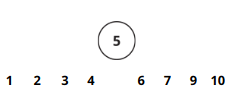
\includegraphics[scale=0.7]{figures/binaria/passo1.png}
    	\label{fig:bubble_sort_example}
    \end{figure}
    
    \item A subárvore esquerda contém os números menores que 5 (\textbf{1, 2, 3, 4}) e a da direita contém os números maiores que 5 (\textbf{6, 7, 9, 10})
    \begin{itemize}
        \item O elemento central (\textbf{2}) é escolhido como a raiz da subárvore esquerda.
        \item O elemento central (\textbf{7}) é escolhido como a raiz da subárvore direita.
    \end{itemize}
    
    \begin{figure}[!ht]
	\centering
	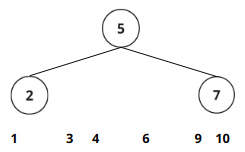
\includegraphics[scale=0.7]{figures/binaria/passo2.png}
	\label{fig:bubble_sort_example}
    \end{figure}
    
    \item Repetimos o processo a partir dos nós 2 e 7
    \begin{itemize}
        \item A subárvore esquerda de 2 contém os números menores que 2 (\textbf{1}) e a da direita contém os números maiores que 2 (\textbf{3, 4})
        \item (\textbf{1}) é escolhido como raíz da árvore esquerda de 2
        \item A subárvore esquerda de 7 contém os números menores que 7 (\textbf{6}) e a da direita contém os números maiores que 7 (\textbf{9, 10})
        \item (\textbf{6}) é escolhido como raíz da árvore esquerda de 7
    \end{itemize}
    
    \begin{figure}[!ht]
	\centering
	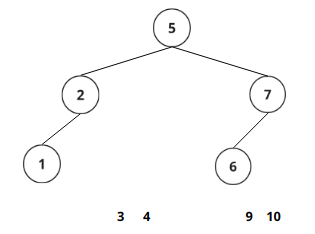
\includegraphics[scale=0.7]{figures/binaria/passo3.png}
	\label{fig:bubble_sort_example}
    \end{figure}
    
    \item Finalizamos a árvore
    \begin{itemize}
        \item O elemento central (\textbf{3}) da árvore direita de 2 é escolhido como a raiz da subárvore direita.
        \item Como (\textbf{4}) é maior que 3, ele será a  raiz da subárvore direita de 3.
        \item O elemento central (\textbf{9}) da árvore direita de 7 é escolhido como a raiz da subárvore direita.
        \item Como (\textbf{10}) é maior que 9, ele será a raiz da subárvore direita de 9.
    \end{itemize}

    \begin{figure}[H]
	\centering
	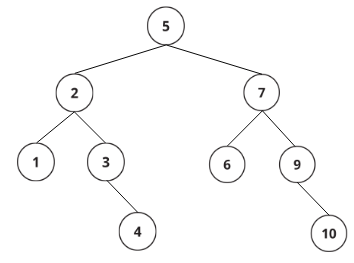
\includegraphics[scale=0.7]{figures/binaria/passo4.png}
	\label{fig:bubble_sort_example}
    \end{figure}
\end{enumerate}

\section*{Implementação em C++}

\subsection*{1. Estrutura do Nó}
\begin{algorithm}[H]
\caption{Estrutura do Nó}
\begin{algorithmic}[1]
\State \textbf{typedef struct nodo} 
\State \quad \textbf{int} chave
\State \quad \textbf{struct nodo*} esq
\State \quad \textbf{struct nodo*} dir
\State \quad Construtor: \textbf{nodo(int chaveNovoNo)}
\State \quad \quad chave $\gets$ chaveNovoNo
\State \quad \quad esq $\gets$ nullptr
\State \quad \quad dir $\gets$ nullptr
\end{algorithmic}
\end{algorithm}

\subsection*{2. Inserção}
\begin{algorithm}[H]
\caption{Inserir}
\begin{algorithmic}[1]
\Function{inserir}{origem, chaveNovoNo}
    \If{origem = nullptr}
        \State \Return novo nó(chaveNovoNo)
    \EndIf
    \If{chaveNovoNo = origem.chave}
        \State \Return origem
    \ElsIf{chaveNovoNo $<$ origem.chave}
        \State origem.esq $\gets$ \Call{inserir}{origem.esq, chaveNovoNo}
    \Else
        \State origem.dir $\gets$ \Call{inserir}{origem.dir, chaveNovoNo}
    \EndIf
    \State \Return origem
\EndFunction
\end{algorithmic}
\end{algorithm}

\subsection*{3. Percurso Pré-Ordem}
\begin{algorithm}[H]
\caption{Percurso Pré-Ordem}
\begin{algorithmic}[1]
\Function{pre\_ordem}{pt}
    \If{pt $\neq$ nullptr}
        \State \textbf{print} pt.chave
        \State \Call{pre\_ordem}{pt.esq}
        \State \Call{pre\_ordem}{pt.dir}
    \EndIf
\EndFunction
\end{algorithmic}
\end{algorithm}

\subsection*{4. Percurso Ordem Simétrica}
\begin{algorithm}[H]
\caption{Percurso Ordem Simétrica}
\begin{algorithmic}[1]
\Function{ordem\_simetrica}{pt}
    \If{pt $\neq$ nullptr}
        \State \Call{ordem\_simetrica}{pt.esq}
        \State \textbf{print} pt.chave
        \State \Call{ordem\_simetrica}{pt.dir}
    \EndIf
\EndFunction
\end{algorithmic}
\end{algorithm}

\subsection*{5. Percurso Pós-Ordem}
\begin{algorithm}[H]
\caption{Percurso Pós-Ordem}
\begin{algorithmic}[1]
\Function{pos\_ordem}{pt}
    \If{pt $\neq$ nullptr}
        \State \Call{pos\_ordem}{pt.esq}
        \State \Call{pos\_ordem}{pt.dir}
        \State \textbf{print} pt.chave
    \EndIf
\EndFunction
\end{algorithmic}
\end{algorithm}

\subsection*{6. Auxiliar em Nível}
\begin{algorithm}[H]
\caption{Auxiliar em Nível}
\begin{algorithmic}[1]
\Function{auxiliar\_em\_nivel}{no, nivel, resultados}
    \If{no = nullptr}
        \State \Return
    \EndIf
    \If{\textbf{size}(resultados) = nivel}
        \State \textbf{add} nova lista em resultados
    \EndIf
    \State resultados[nivel].\textbf{push\_back}(no.chave)
    \State \Call{auxiliar\_em\_nivel}{no.esq, nivel+1, resultados}
    \State \Call{auxiliar\_em\_nivel}{no.dir, nivel+1, resultados}
\EndFunction
\end{algorithmic}
\end{algorithm}

\subsection*{7. Percurso por Nível}
\begin{algorithm}[H][H]
\caption{Percurso por Nível}
\begin{algorithmic}[1]
\Function{em\_nivel}{no}
    \State resultados $\gets$ lista vazia
    \State \Call{auxiliar\_em\_nivel}{no, 0, resultados}
    \For{cada nivel em resultados}
        \For{cada chave em nivel}
            \State \textbf{print} chave
        \EndFor
        \State \textbf{print} "|"
    \EndFor
\EndFunction
\end{algorithmic}
\end{algorithm}

\subsection*{8. Busca}
\begin{algorithm}[H]
\caption{Busca}
\begin{algorithmic}[1]
\Function{busca}{raiz, chave}
    \If{raiz = nullptr OR raiz.chave = chave}
        \State \Return raiz
    \ElsIf{chave $<$ raiz.chave}
        \State \Return \Call{busca}{raiz.esq, chave}
    \Else
        \State \Return \Call{busca}{raiz.dir, chave}
    \EndIf
\EndFunction
\end{algorithmic}
\end{algorithm}

\subsection*{9. Busca Iterativa}
\begin{algorithm}[H]
\caption{Busca Iterativa}
\begin{algorithmic}[1]
\Function{busca\_iterativa}{raiz, chave}
    \While{raiz $\neq$ nullptr AND raiz.chave $\neq$ chave}
        \If{chave $<$ raiz.chave}
            \State raiz $\gets$ raiz.esq
        \Else
            \State raiz $\gets$ raiz.dir
        \EndIf
    \EndWhile
    \State \Return raiz
\EndFunction
\end{algorithmic}
\end{algorithm}

\subsection*{10. Encontrar Mínimo}
\begin{algorithm}[H]
\caption{Encontra Mínimo}
\begin{algorithmic}[1]
\Function{encontra\_minimo}{raiz}
    \While{raiz $\neq$ nullptr AND raiz.esq $\neq$ nullptr}
        \State raiz $\gets$ raiz.esq
    \EndWhile
    \State \Return raiz
\EndFunction
\end{algorithmic}
\end{algorithm}

\subsection*{11. Remoção}
\begin{algorithm}[H]
\caption{Remover}
\begin{algorithmic}[1]
\Function{remover}{root, chave}
    \If{root = nullptr}
        \State \Return nullptr
    \ElsIf{chave $<$ root.chave}
        \State root.esq $\gets$ \Call{remover}{root.esq, chave}
    \ElsIf{chave $>$ root.chave}
        \State root.dir $\gets$ \Call{remover}{root.dir, chave}
    \Else
        \If{root.esq = nullptr AND root.dir = nullptr}
            \State \textbf{delete} root
            \State \Return nullptr
        \ElsIf{root.esq = nullptr}
            \State temp $\gets$ root.dir
            \State \textbf{delete} root
            \State \Return temp
        \ElsIf{root.dir = nullptr}
            \State temp $\gets$ root.esq
            \State \textbf{delete} root
            \State \Return temp
        \Else
            \State temp $\gets$ \Call{encontra\_minimo}{root.dir}
            \State root.chave $\gets$ temp.chave
            \State root.dir $\gets$ \Call{remover}{root.dir, temp.chave}
        \EndIf
    \EndIf
    \State \Return root
\EndFunction
\end{algorithmic}
\end{algorithm}

\end{document}

